\section{Лекція 5: Умовні оператори}
 
 \subsection{Логічні висновки} 
\begin{frame}
% \frametitle{Логічні висновки}
\begin{itemize}
  \item True - істина
  \item False - брехня
 \end{itemize}

\begin{figure}
\begin{center}
 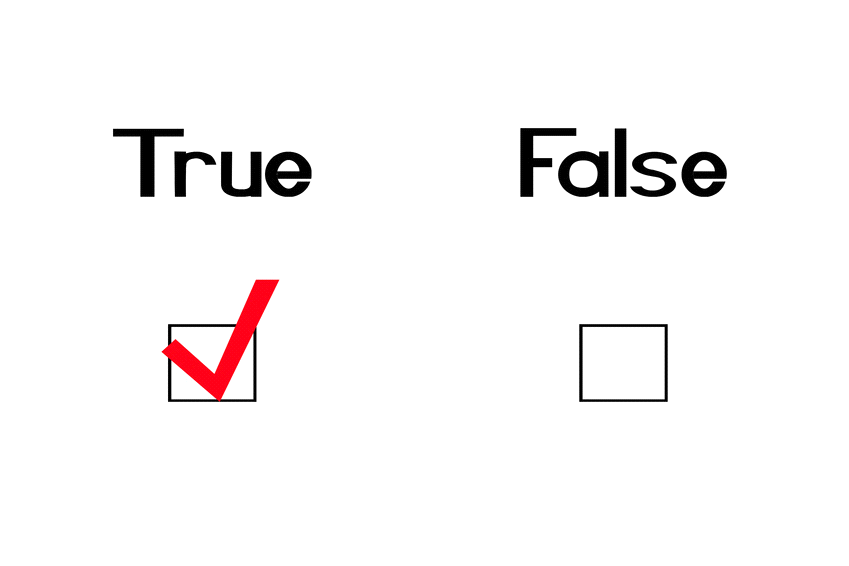
\includegraphics[width=0.4\textwidth]{pictures/TrueFalse.png}
\caption{True або False ?}
\label{TrueFalse} 
\end{center}
\end{figure}
\end{frame}

 \subsection{Логічні вирази} 
\begin{frame}
% \frametitle{Логічні вирази}

\begin{table}
  \caption{Логічні вирази}
  \label{tab:}

  \begin{center}
    \begin{tabular}{|c|c|}
    \hline
      \textbf{Оператор} & \textbf{Значення} \\
    \hline  
      < & менше \\
    \hline
      >  & більше\\
    \hline
      <=  & менше або дорівнює \\
    \hline
      >=  & більше або дорівнює\\
    \hline
      ==  & дорівнює \\
    \hline
      !=  & не дорівнює \\
    \hline
    \end{tabular}
  \end{center}
\end{table}

\end{frame}

 \subsection{Логічні оператори} 
\begin{frame}
% \frametitle{Логічні оператори}
\begin{table}
  \caption{Логічні оператори}
  \label{tab:}

  \begin{center}
    \begin{tabular}{|c|c|c|}
    \hline
      \textbf{Оператор} & \textbf{Значення} & \textbf{Пріоритет} \\
    \hline  
      or & або & 1 \\
    \hline
      and & та & 2 \\
    \hline
      not & ні & 3 \\
    \hline
    \end{tabular}
  \end{center}
\end{table}
\end{frame}

%  \subsection{Логічні оператори} 
\begin{frame}
% \frametitle{Робота з логічними виразами}
\begin{itemize}
  \item Перевірка на парність/непарність;
  \item Перевірка на потрапляння/непотрапляння в інтервал;
  \item Функція bool().
 \end{itemize}
\end{frame}

 \subsection{Умовний оператор} 
\begin{frame}
% \frametitle{Логічні висновки}
if - умовний оператор (оператор розгалуження).

% \begin{center}
\huge{if вираз:

~~~~операції}


\begin{flushleft}
\normalsize
Програма оцінює значення `вираз`, яке може дорівнювати True або False. Програма виконає операції тільки якщо вираз = True. Якщо вираз = False, цей шматок коду не буде виконуватись.
\end{flushleft}
% \end{center}
\end{frame}

\begin{frame}
% \frametitle{Логічні висновки}
\huge{if вираз:

~~~~операції 1

else:

~~~~операції 2}


\begin{flushleft}
\normalsize
Операції 1 виконуються тільки якщо вираз істинний (дорівнює True). Якщо вираз дорівнює False, виконуються операції 2. Для розділення цих блоків використовуються відступи.
\end{flushleft}
% \end{center}
\end{frame}


\begin{frame}
% \frametitle{Логічні висновки}
\huge{if вираз 1:

~~~~операції 1

elif вираз 2:

~~~~операції 2

else:

~~~~операції 3}

\end{frame}

 \subsection{Використання умовного оператору} 
\begin{frame}
% \frametitle{Логічні висновки}
\begin{figure}
\begin{center}
 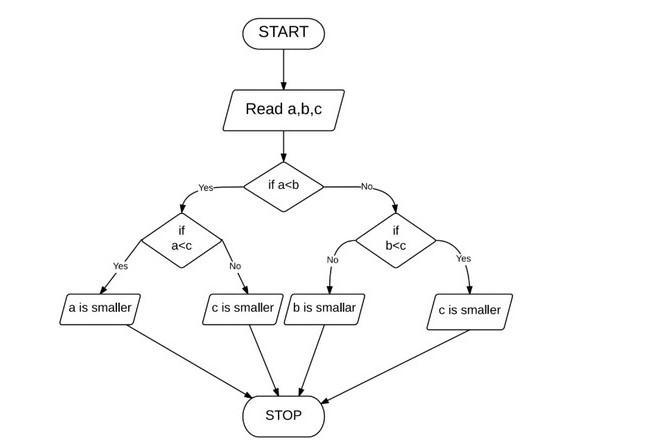
\includegraphics[width=0.6\textwidth]{pictures/find_min.jpg}
\caption{Алгоритм знаходження мінімального із трьох чисел}
\label{find_min} 
\end{center}
\end{figure}
\end{frame}

 \subsection{Тернарний умовний оператор} 
\begin{frame}
% % \frametitle{Логічні висновки}
У Python існує конструкція, яка за своєю дією аналогічна конструкції if-else, але є виразом. Вона називається тернарним оператором.

\Large{\texttt{значення\_1 if умова else значення\_2}}

Тернарний оператор повертає результат.
\end{frame}
